\chapter{धातुएँ: अम्लों के साथ अभिक्रियाएँ और संक्षारण}\label{ch:g9:metals-acids-corrosion}

एक बंदरगाह में मछली पकड़ने वाली एक पुरानी नाव का स्टील का ढाँचा नारंगी \omterm{def:g9:metals-acids-corrosion:corrosion}{जंग} की
धारियों से भरा है। घाट पर ज़िंक-लेपित एक फाटक तीस साल से बारिश में खड़ा है
और अब भी हल्की धूसर चमक लिए है। एक संग्रहालय में तीन हज़ार साल तक दबी रही
सोने की एक अँगूठी उतनी ही चमकदार है जितनी बनने के दिन थी। सभी धातुएँ दुनिया
का सामना एक ही ढंग से नहीं करतीं: कुछ पर पानी, \omterm{def:g4:air-a-mixture-of-gases:air}{वायु} और अम्ल आक्रमण करते हैं,
कुछ पर लगभग बिल्कुल नहीं।

\begin{recall}
\omterm{def:g9:ions:ion}{आयन} आवेशित \omterm{def:g7:atoms-and-molecules:atom}{परमाणु} हैं; धातुएँ \ce{Fe^{2+}}, \ce{Zn^{2+}}, \ce{Al^{3+}} जैसे
\omterm{def:g9:ions:ion}{धनायन} देती हैं, जिन्हें \omterm{def:g9:ions:precipitate}{अवक्षेपण} परीक्षणों से पहचाना जाता है
(\cref{ch:g9:ions})। \omterm{def:g9:acids-bases-ph:acidic}{अम्लीय विलयन} में बहुत-से \ce{H+(aq)} \omterm{def:g9:ions:ion}{आयन} होते हैं
(\cref{ch:g9:acids-bases-ph})। हाइड्रोजन परखनली के मुँह पर तीखी `पॉप' की आवाज़
के साथ \omterm{def:g4:what-a-fire-needs:burning}{जलती} है (\cref{ch:g7:identifying-substances})।
\end{recall}

\begin{omfigure}
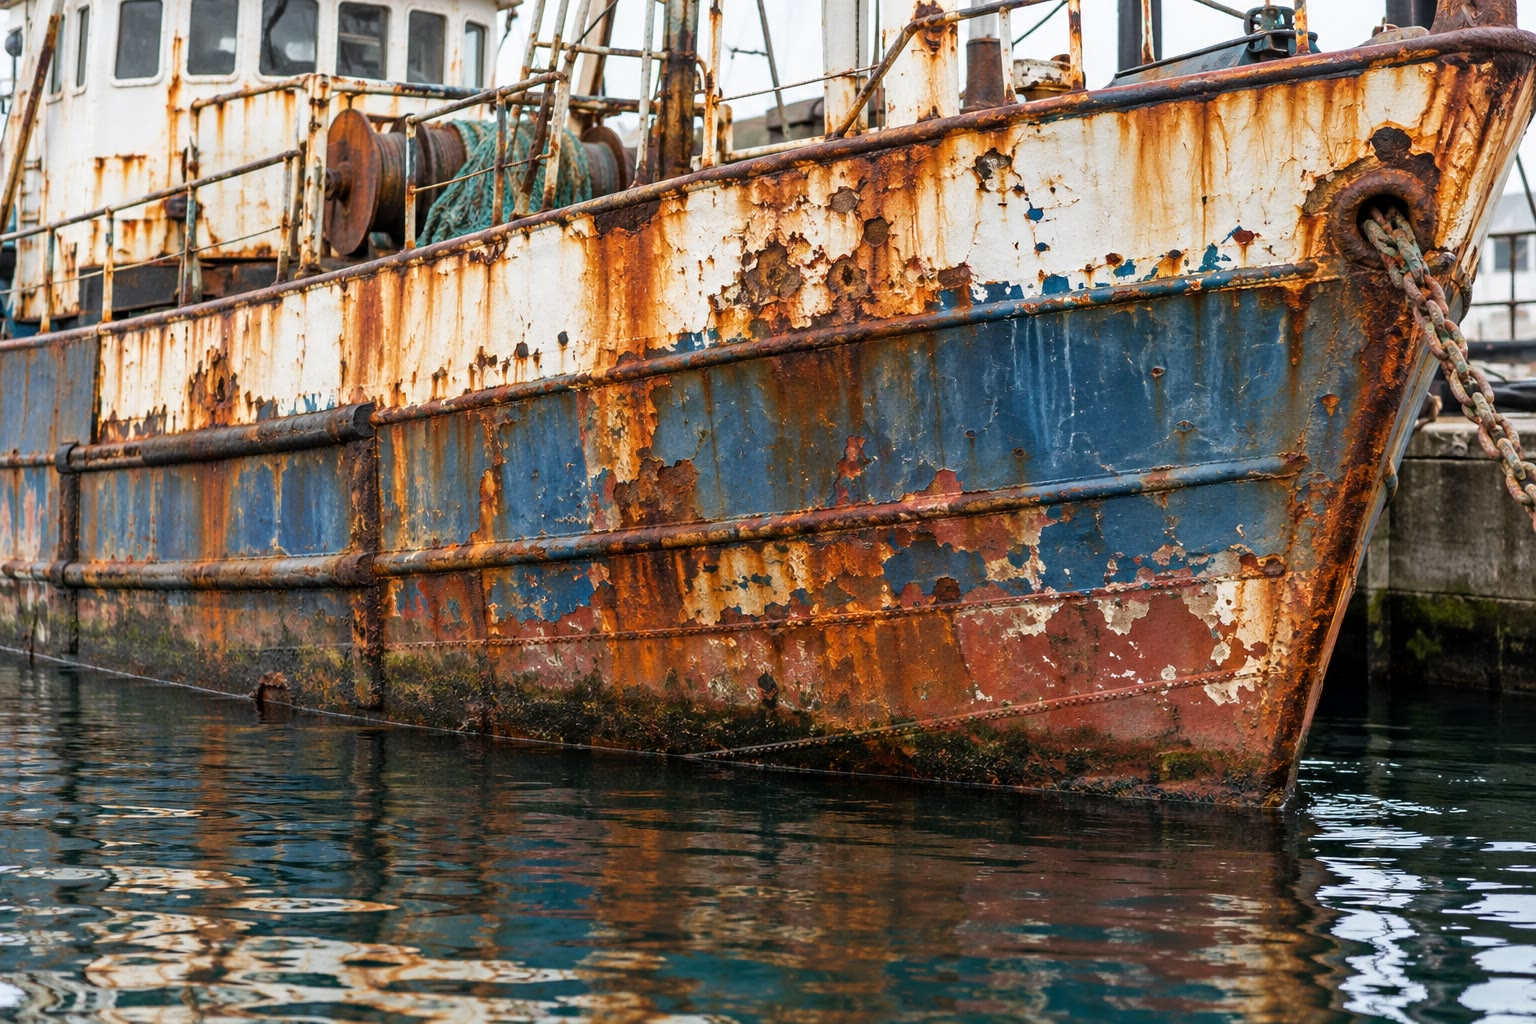
\includegraphics[width=0.55\linewidth]{images/book1/ai/g9-rusty-hull.jpg}

{\small एक पुरानी नाव का ढाँचा: स्टील में \omterm{def:g9:metals-acids-corrosion:corrosion}{जंग} लग रहा है।}
\end{omfigure}

\section{हाइड्रोक्लोरिक अम्ल में धातुएँ}

\begin{inthelab}[अम्ल में तीन धातुएँ]
शिक्षक तनु हाइड्रोक्लोरिक अम्ल से भरी तीन परखनलियों में लोहे, ज़िंक और ताँबे का एक-एक
छोटा टुकड़ा डालते हैं। लोहे और ज़िंक से बुलबुले उठते हैं, लोहे से धीरे-धीरे,
ज़िंक से तेज़ी से, और धातुएँ धीरे-धीरे ग़ायब होती जाती हैं; ताँबे को कुछ नहीं
होता। एक छोटी नली में इकट्ठी की गई गैस तीखी `पॉप' की आवाज़ देती है: वह
हाइड्रोजन है। सोडियम हाइड्रॉक्साइड के साथ पहली नली का द्रव हरा \omterm{def:g9:ions:precipitate}{अवक्षेप} देता है
(\ce{Fe^{2+}} \omterm{def:g9:ions:ion}{आयन}), दूसरी नली का सफ़ेद (\ce{Zn^{2+}} \omterm{def:g9:ions:ion}{आयन})।
\end{inthelab}

\begin{omfigure}
\begin{tikzpicture}[font=\small, scale=1.2]
  \foreach \k/\m/\c/\bub in {0/लोहा/black!45/4, 1/ज़िंक/black!25/9, 2/ताँबा/orange!60!brown/0} {
    \pic[transform shape] at (\k*2.4,0) {testtube={0.55}{omWater!70}};
    \fill[\c] (\k*2.4-0.13,0.08) rectangle (\k*2.4+0.13,0.35);
    \ifnum\bub>0
      \foreach \j in {1,...,\bub} {
        \pgfmathsetmacro\yy{0.45+0.12*\j}
        \pgfmathsetmacro\xx{\k*2.4+0.1*sin(97*\j)}
        \draw[black!55] (\xx,\yy) circle (0.035);
      }
    \fi
    \node[anchor=north, align=center] at (\k*2.4,-0.15) {\m};
  }
  \node[anchor=north, align=center, font=\footnotesize] at (0,-0.6) {बुलबुले, धीरे-धीरे};
  \node[anchor=north, align=center, font=\footnotesize] at (2.4,-0.6) {बुलबुले, तेज़ी से};
  \node[anchor=north, align=center, font=\footnotesize] at (4.8,-0.6) {कोई अभिक्रिया नहीं};
\end{tikzpicture}

{\small तनु हाइड्रोक्लोरिक अम्ल में लोहा, ज़िंक और ताँबा: लोहा और ज़िंक
हाइड्रोजन देते हैं; ताँबा अभिक्रिया नहीं करता।}
\end{omfigure}

\begin{proposition}[धातु और अम्ल]\label{prop:g9:metals-acids-corrosion:acid}
बहुत-सी धातुएँ --- लोहा, ज़िंक, ऐलुमिनियम, मैग्नीशियम --- अम्ल के \ce{H+}
\omterm{def:g9:ions:ion}{आयनों} के साथ अभिक्रिया करती हैं: धातु धातु-आयनों के रूप में ग़ायब हो जाती है, जो
घुले रहते हैं, और हाइड्रोजन गैस निकलती है। ताँबा, चाँदी और सोना हाइड्रोक्लोरिक
अम्ल के साथ अभिक्रिया नहीं करते।
\end{proposition}

\section{आयनों के साथ समीकरण लिखना}

\begin{definition}[दर्शक आयन]\label{def:g9:metals-acids-corrosion:spectator}
जो \omterm{def:g9:ions:ion}{आयन} अभिक्रिया के दौरान विलयन में मौजूद रहता है पर उसमें भाग नहीं लेता, और
अंत में बिना बदले मिलता है, वह \emph{दर्शक
आयन}\index{दर्शक आयन} है। उसे समीकरण में नहीं लिखा जाता।
\end{definition}

\begin{example}[हाइड्रोक्लोरिक अम्ल में लोहा और ज़िंक]\label{ex:g9:metals-acids-corrosion:iron}
हाइड्रोक्लोरिक अम्ल में \ce{H+(aq)} और \ce{Cl-(aq)} \omterm{def:g9:ions:ion}{आयन} होते हैं।
क्लोराइड \omterm{def:g9:ions:ion}{आयन} अंत में बिना बदले मिलते हैं: वे दर्शक हैं।
समीकरण ये हैं:
\[
  \ce{Fe(s) + 2H+(aq) -> Fe^{2+}(aq) + H2(g)}, \qquad
  \ce{Zn(s) + 2H+(aq) -> Zn^{2+}(aq) + H2(g)}.
\]
ये \omterm{def:g7:atoms-and-molecules:atom}{परमाणुओं} और आवेशों, दोनों को संतुलित करते हैं: हर ओर $+2$।
\end{example}

\begin{method}[अम्ल के साथ धातु का समीकरण लिखना]\label{met:g9:metals-acids-corrosion:write}
\begin{enumerate}
  \item \omterm{def:g7:chemical-reactions:reactant}{अभिकारक}: धातु (s) और \ce{H+(aq)} \omterm{def:g9:ions:ion}{आयन}।
  \item उत्पाद: अपने सामान्य आवेश के साथ धातु-आयन (aq), और
        हाइड्रोजन \ce{H2(g)}।
  \item \omterm{def:g7:atoms-and-molecules:atom}{परमाणुओं} को संतुलित करो, फिर जाँचो कि कुल आवेश दोनों ओर
        बराबर है।
\end{enumerate}
ऐलुमिनियम के लिए: \ce{2Al(s) + 6H+(aq) -> 2Al^{3+}(aq) + 3H2(g)}; हर ओर
आवेश $+6$।
\end{method}

\begin{safety}{\ghs[0.8cm]{GHS02}\ghs[0.8cm]{GHS04}}
% ledger: ghs:H2
निकलने वाली हाइड्रोजन अत्यंत ज्वलनशील है। अभिक्रिया छोटी परखनलियों में, शिक्षक
द्वारा, किसी भी लौ से दूर की जाती है --- सिवाय उस लौ के जो `पॉप' परीक्षण
के लिए इस्तेमाल होती है।
\end{safety}

\section{संक्षारण}

\begin{definition}[संक्षारण और जंग]\label{def:g9:metals-acids-corrosion:corrosion}
\emph{संक्षारण}\index{संक्षारण} आस-पास के पदार्थों --- ऑक्सीजन, पानी, अम्ल,
लवण --- द्वारा किसी धातु पर होने वाला धीमा आक्रमण है, जो धातु को \omterm{def:g9:ions:ion}{आयनों} में या
ऑक्साइड जैसे यौगिकों में बदल देता है। लोहे और स्टील के संक्षारण से
\emph{जंग}\index{जंग} बनता है, एक भूरा, भुरभुरा, जलयोजित
आयरन ऑक्साइड, जो पपड़ी बनकर उतर जाता है और आक्रमण को और गहराई तक जाने देता है।
\end{definition}

\begin{proposition}[लोहे को जंग लगने के लिए क्या चाहिए]\label{prop:g9:metals-acids-corrosion:needs}
लोहे में \omterm{def:g9:metals-acids-corrosion:corrosion}{जंग} तभी लगता है जब ऑक्सीजन और पानी दोनों उस तक पहुँचें। पानी में घुला
नमक, जैसे सर्दियों में नमक छिड़की गई सड़कों पर या समुद्र के पास, \omterm{def:g9:metals-acids-corrosion:corrosion}{जंग}
लगने को तेज़ कर देता है।
\end{proposition}

\begin{inthelab}[तीन कीलें, एक हफ़्ता]
लोहे की तीन साफ़ कीलें तीन परखनलियों में रखी जाती हैं: पहली सूखी \omterm{def:g4:air-a-mixture-of-gases:air}{वायु} के साथ
और एक शोषक पदार्थ के साथ जो जलवाष्प हटा देता है; दूसरी ऐसे पानी में जिसे उबालकर
उसकी घुली हुई \omterm{def:g4:air-a-mixture-of-gases:air}{वायु} निकाल दी गई है, और जिस पर तेल की परत है; तीसरी आधी नल के
पानी में, आधी \omterm{def:g4:air-a-mixture-of-gases:air}{वायु} में। एक हफ़्ते बाद केवल तीसरी कील में
\omterm{def:g9:metals-acids-corrosion:corrosion}{जंग} लगा होता है।
\end{inthelab}

\begin{omfigure}
\begin{tikzpicture}[font=\small, scale=1.2]
  % tube 1: dry air, drying agent
  \pic[transform shape] at (0,0) {testtube={0.18}{white!80!black}};
  \foreach \x/\y in {-0.12/0.15,0.08/0.12,-0.02/0.3,0.12/0.32,-0.14/0.42,0.03/0.48}
    \fill[black!35] (\x,\y) circle (0.05);
  \fill[black!45] (-0.03,1.0) rectangle (0.03,2.4);
  \fill[black!45] (-0.09,2.4) rectangle (0.09,2.48);
  \fill[black!60] (-0.3,2.8) rectangle (0.3,3.1);
  \node[anchor=north, align=center] at (0,-0.15) {सूखी वायु:\\ जंग नहीं};
  % tube 2: boiled water under oil
  \pic[transform shape] at (2.6,0) {testtube={0.7}{omWater!80}};
  \fill[yellow!55!orange!60] (2.36,1.85) rectangle (2.84,2.1);
  \fill[black!45] (2.57,0.3) rectangle (2.63,1.7);
  \fill[black!45] (2.51,1.7) rectangle (2.69,1.78);
  \fill[black!60] (2.3,2.8) rectangle (2.9,3.1);
  \node[anchor=north, align=center] at (2.6,-0.15) {बिना वायु का पानी:\\ जंग नहीं};
  % tube 3: water and air
  \pic[transform shape] at (5.2,0) {testtube={0.4}{omWater!80}};
  \fill[black!45] (5.17,0.3) rectangle (5.23,2.2);
  \fill[black!45] (5.11,2.2) rectangle (5.29,2.28);
  \fill[orange!60!brown] (5.15,0.9) rectangle (5.25,1.5);
  \node[anchor=north, align=center] at (5.2,-0.15) {पानी और वायु:\\ जंग};
  \draw[<-, omProp, thick] (-0.15,0.3) -- (-0.9,0.7) node[left, text=black, font=\footnotesize] {शोषक};
  \draw[<-, omProp, thick] (2.85,1.98) -- (3.6,2.4) node[right, text=black, font=\footnotesize] {तेल};
\end{tikzpicture}

{\small तीन कीलों वाला प्रयोग: लोहे में \omterm{def:g9:metals-acids-corrosion:corrosion}{जंग} वहीं लगता है जहाँ पानी और ऑक्सीजन
एक साथ पहुँचते हैं, यहाँ पानी की सतह पर।}
\end{omfigure}

\begin{example}[ऐलुमिनियम और ताँबा ख़ुद को बचाते हैं]\label{ex:g9:metals-acids-corrosion:protect}
\omterm{def:g4:air-a-mixture-of-gases:air}{वायु} की ऑक्सीजन ऐलुमिनियम पर तुरंत आक्रमण करती है, पर बनी हुई ऑक्साइड की पतली
परत धातु से चिपक जाती है और उसे \omterm{def:g4:air-a-mixture-of-gases:air}{वायु} से बंद कर देती है: ऐलुमिनियम की खिड़कियों
के चौखटे दशकों तक चलते हैं। ताँबा, जिस पर \omterm{def:g4:air-a-mixture-of-gases:air}{वायु}, पानी और कार्बन डाइऑक्साइड धीरे-धीरे
आक्रमण करते हैं, एक हरी पपड़ी से ढक जाता है, जिसे पैटिना कहते हैं, जो भी चिपकी
रहती है और नीचे की धातु की रक्षा करती है। इसके विपरीत, \omterm{def:g9:metals-acids-corrosion:corrosion}{जंग} पपड़ी बनकर
उतर जाता है।
\end{example}

\begin{omfigure}
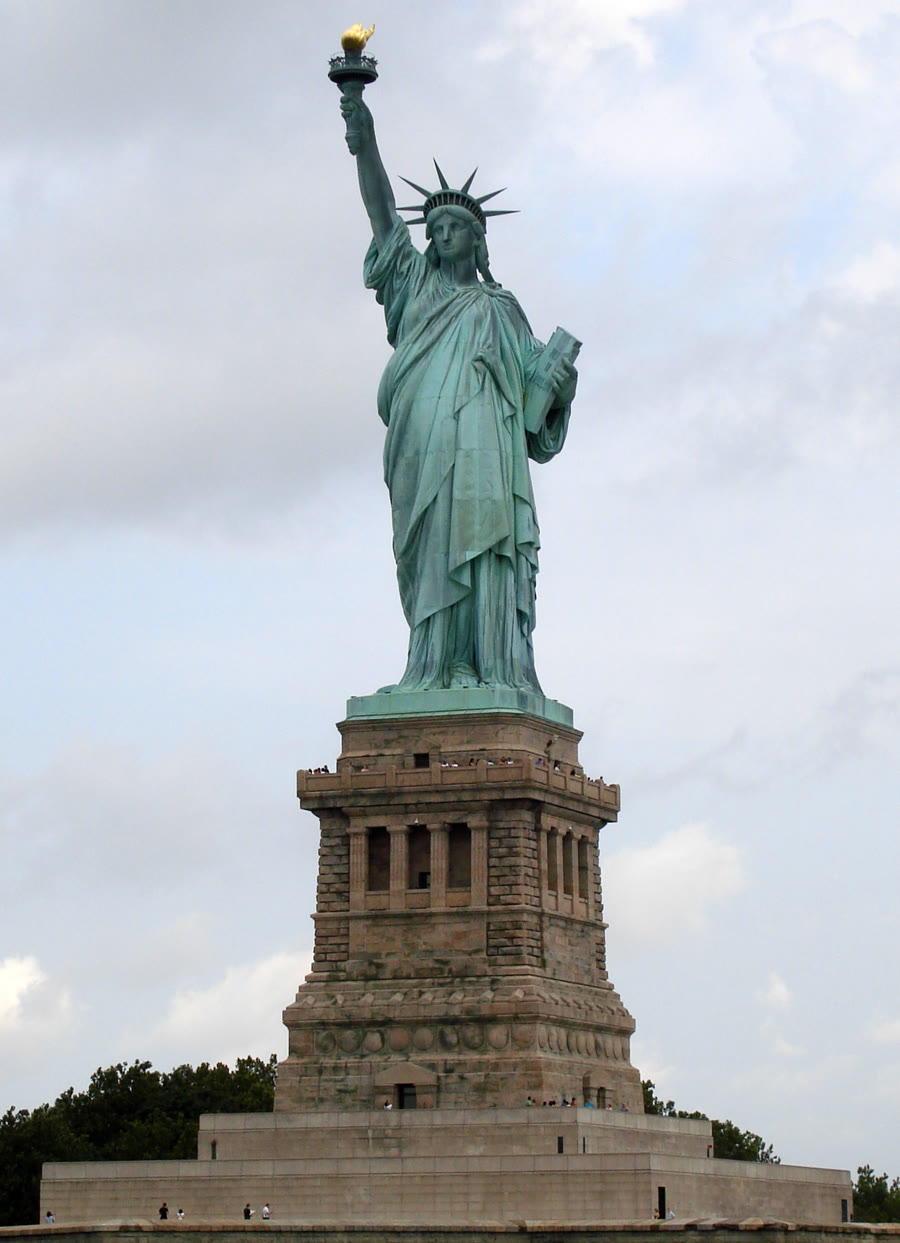
\includegraphics[height=6cm]{images/book1/statue-patina.jpg}

{\small स्टैच्यू ऑफ़ लिबर्टी: उसकी ताँबे की त्वचा हरे पैटिना से ढकी है।
फ़ोटो: एलकोबोला, सार्वजनिक डोमेन।}
\end{omfigure}

\section{धातुओं की रक्षा}

\begin{definition}[यशदलेपन]\label{def:g9:metals-acids-corrosion:galvanising}
\emph{यशदलेपन}\index{यशदलेपन} यानी स्टील को पिघले हुए ज़िंक में डुबोकर उस पर
ज़िंक की परत चढ़ाना। \omterm{def:g4:air-a-mixture-of-gases:air}{वायु} और पानी नीचे के स्टील के बजाय ज़िंक पर आक्रमण
करते हैं: जहाँ परत खुरच भी गई हो, वहाँ भी पास का ज़िंक पहले संक्षारित होता
है और स्टील बच जाता है।
\end{definition}

\begin{proposition}[लोहे और स्टील की रक्षा के तरीके]\label{prop:g9:metals-acids-corrosion:ways}
\begin{itemize}
  \item पानी और \omterm{def:g4:air-a-mixture-of-gases:air}{वायु} को दूर रखना: पेंट, तेल, ग्रीस, \omterm{def:g8:plastics:plastic}{प्लास्टिक} की परत;
  \item \omterm{def:g9:metals-acids-corrosion:galvanising}{यशदलेपन}: ज़िंक की परत, जो स्टील की जगह संक्षारित होती है;
  \item स्टेनलेस स्टील का उपयोग, जो लोहे और क्रोमियम की एक मिश्रातु है और
        ऑक्साइड की एक पतली, बंद करने वाली परत से ख़ुद की रक्षा करती है;
  \item जहाज़ों के ढाँचों पर ज़िंक के गुटके लगाना: स्टील के बजाय ज़िंक धीरे-धीरे
        घिसता जाता है, और समय-समय पर बदला जाता है (यह कैसे काम करता है, यह
        विश्वविद्यालय के एक खंड में समझाया गया है)।
\end{itemize}
\end{proposition}

\begin{omfigure}
\begin{minipage}[b]{0.52\linewidth}\centering
\begin{tikzpicture}[font=\small]
  \fill[black!35] (0,0) rectangle (5,0.8);
  \fill[black!15] (0,0.8) rectangle (2.2,1.1);
  \fill[black!15] (2.8,0.8) rectangle (5,1.1);
  \fill[omWater!80] (1.6,1.1) rectangle (3.4,1.35);
  \fill[omWater!80] (2.2,0.8) rectangle (2.8,1.1);
  \draw[black!60] (0,0) rectangle (5,0.8);
  \foreach \x in {1.95,2.1} \draw[->, omProp, thick] (\x,1.25) -- (\x+0.05,1.7);
  \node[anchor=west, font=\footnotesize] at (5.1,0.4) {स्टील};
  \node[anchor=west, font=\footnotesize] at (5.1,0.95) {ज़िंक की परत};
  \node[anchor=south, font=\footnotesize, align=center] at (2.0,1.75) {ज़िंक आयन\\ पानी में जाते हैं};
  \node[anchor=north, font=\footnotesize, align=center] at (2.5,-0.05) {खरोंच: स्टील\\ खुल गया है, पर आस-पास\\ का ज़िंक पहले संक्षारित होता है};
\end{tikzpicture}

{\small खुरची हुई यशदलेपित चादर।}
\end{minipage}\hfill
\begin{minipage}[b]{0.44\linewidth}\centering
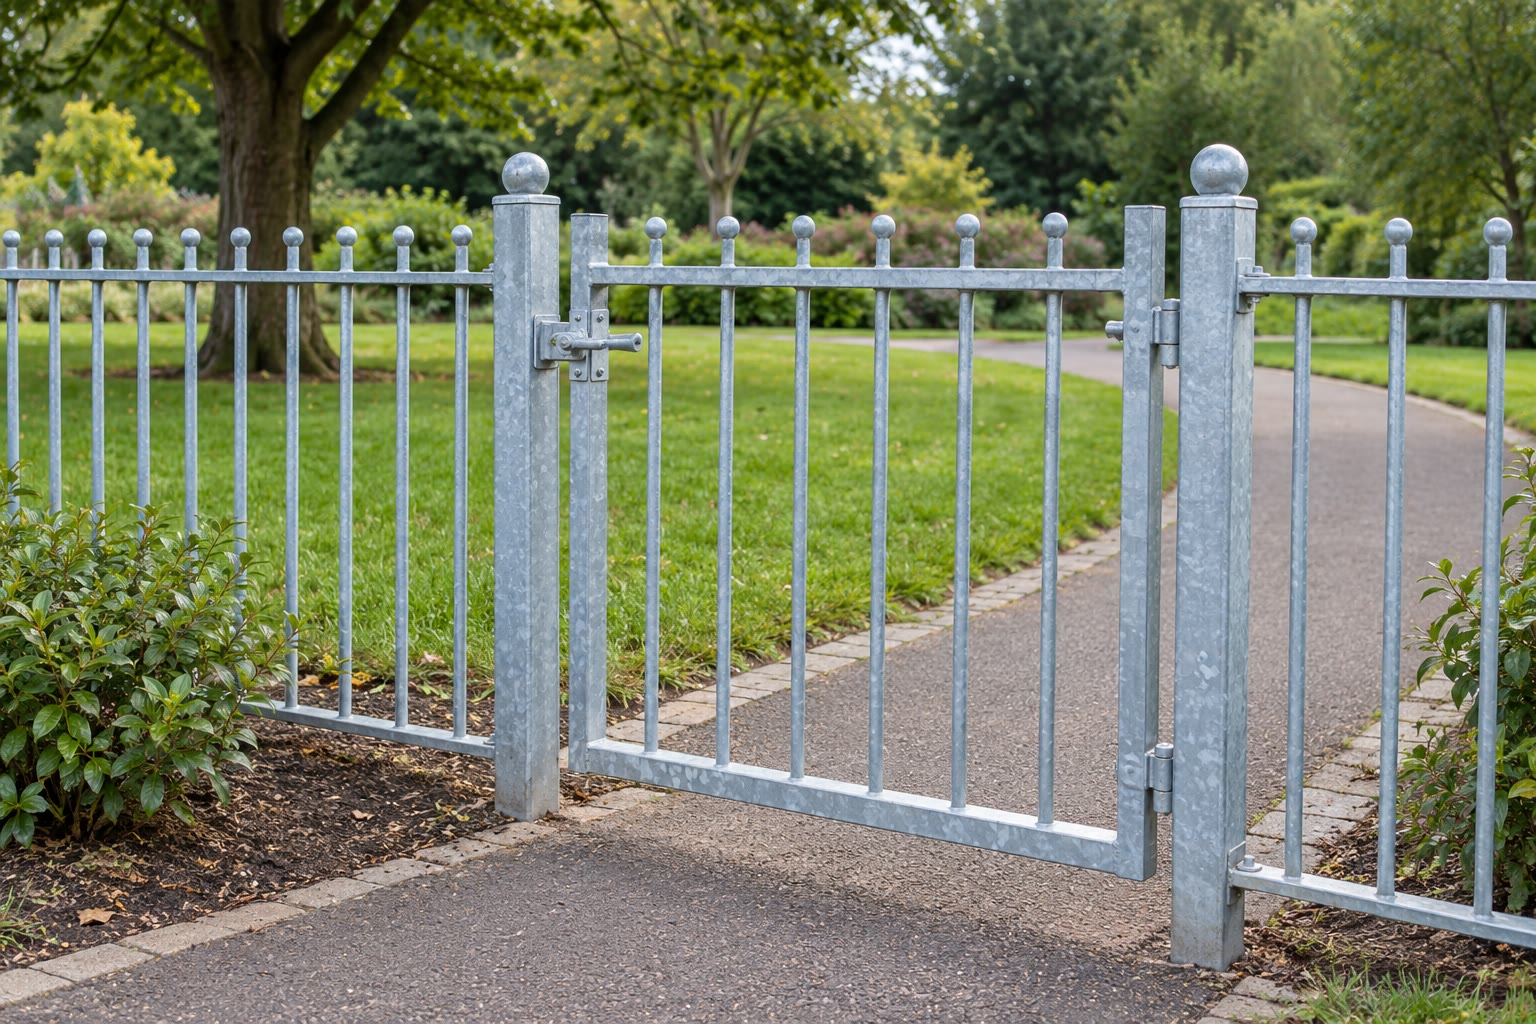
\includegraphics[width=\linewidth,height=4.4cm,keepaspectratio]{images/book1/ai/g9-galvanised-railings.jpg}

{\small यशदलेपित स्टील की रेलिंग।}
\end{minipage}
\end{omfigure}

\section{अभ्यास}

\begin{exercise}[$\star$]\label{exo:g9:metals-acids-corrosion:1}
ज़िंक के हाइड्रोक्लोरिक अम्ल के साथ अभिक्रिया करने पर कौन-सी गैस निकलती है? उसे
कैसे पहचाना जाता है?
\end{exercise}

\begin{exercise}[$\star$]\label{exo:g9:metals-acids-corrosion:2}
इनमें से कौन-सी धातुएँ तनु हाइड्रोक्लोरिक अम्ल के साथ अभिक्रिया करती हैं: लोहा, ताँबा,
ज़िंक, सोना, ऐलुमिनियम?
\end{exercise}

\begin{exercise}[$\star$]\label{exo:g9:metals-acids-corrosion:3}
लोहे को \omterm{def:g9:metals-acids-corrosion:corrosion}{जंग} लगने के लिए क्या चाहिए?
\end{exercise}

\begin{exercise}[$\star$]\label{exo:g9:metals-acids-corrosion:4}
\omterm{def:g9:metals-acids-corrosion:spectator}{दर्शक आयन} क्या है? लोहे के हाइड्रोक्लोरिक अम्ल के साथ अभिक्रिया करने पर \omterm{def:g9:metals-acids-corrosion:spectator}{दर्शक आयन}
का नाम बताओ।
\end{exercise}

\begin{exercise}[$\star\star$]\label{exo:g9:metals-acids-corrosion:5}
किसी अम्ल के \ce{H+} \omterm{def:g9:ions:ion}{आयनों} के साथ मैग्नीशियम की अभिक्रिया का समीकरण लिखो
(मैग्नीशियम \omterm{def:g9:ions:ion}{आयन} \ce{Mg^{2+}} है)। आवेशों की जाँच करो।
\end{exercise}

\begin{exercise}[$\star\star$]\label{exo:g9:metals-acids-corrosion:6}
लोहे के हाइड्रोक्लोरिक अम्ल के साथ अभिक्रिया कर लेने के बाद तुम कैसे दिखाओगे कि
विलयन में आयरन(II) \omterm{def:g9:ions:ion}{आयन} हैं?
\end{exercise}

\begin{exercise}[$\star\star$]\label{exo:g9:metals-acids-corrosion:7}
तीन कीलों वाला चित्र देखो। दूसरी नली का पानी क्यों उबाला गया है और उस पर
तेल क्यों डाला गया है?
\end{exercise}

\begin{exercise}[$\star\star$]\label{exo:g9:metals-acids-corrosion:8}
जिस शहर में सर्दियों में सड़कों पर नमक छिड़का जाता है, वहाँ कार में \omterm{def:g9:metals-acids-corrosion:corrosion}{जंग} जल्दी क्यों लगता है?
\end{exercise}

\begin{exercise}[$\star\star$]\label{exo:g9:metals-acids-corrosion:9}
ऐलुमिनियम की खिड़कियों के चौखटे संक्षारित होकर नष्ट क्यों नहीं होते, हालाँकि
ऐलुमिनियम \omterm{def:g4:air-a-mixture-of-gases:air}{वायु} की ऑक्सीजन के साथ अभिक्रिया करता है?
\end{exercise}

\begin{exercise}[$\star\star$]\label{exo:g9:metals-acids-corrosion:10}
स्टील की साइकिल के ढाँचे को \omterm{def:g9:metals-acids-corrosion:corrosion}{जंग} से बचाने के तीन तरीके बताओ।
\end{exercise}

\begin{exercise}[$\star\star\star$]\label{exo:g9:metals-acids-corrosion:11}
किसी अम्ल के \ce{H+} \omterm{def:g9:ions:ion}{आयनों} के साथ ऐलुमिनियम की अभिक्रिया का समीकरण लिखो और
उसकी जाँच करो। 200 ऐलुमिनियम \omterm{def:g7:atoms-and-molecules:atom}{परमाणुओं} से हाइड्रोजन के कितने \omterm{def:g7:atoms-and-molecules:molecule}{अणु} बनते
हैं?
\end{exercise}

\begin{exercise}[$\star\star\star$]\label{exo:g9:metals-acids-corrosion:12}
यशदलेपित स्टील की एक बाल्टी स्टील तक खुरच जाती है। समझाओ कि खरोंच की तली
में स्टील पर लंबे समय तक \omterm{def:g9:metals-acids-corrosion:corrosion}{जंग} क्यों नहीं लगता।
\end{exercise}

\section{समस्या: ज़िंक कितना मोटा है?}

\begin{problem}[{सप्ताहांत समस्या --- यशदलेपित प्लेट की ज़िंक-परत को घोलकर
यह पता करना कि वह कितनी मोटी थी}]
\label{pb:g9:metals-acids-corrosion:1}
% ledger: rho:Zn
\qty{10.0}{cm} भुजा वाली एक वर्गाकार यशदलेपित स्टील प्लेट के दोनों फलकों पर
ज़िंक की परत है (किनारे नगण्य माने जाते हैं)। प्रयोगशाला में शिक्षक
उसे तौलते हैं, \qty{125.6}{g}, फिर उसे ऐसे हाइड्रोक्लोरिक अम्ल में डुबोते हैं
जिसमें एक योज्य है जो अम्ल को स्टील पर आक्रमण करने से रोकता है। बुलबुले
बंद होने पर प्लेट को धोकर, सुखाकर फिर तौला जाता है: \qty{113.5}{g}।
\qty{1}{cm^3} ज़िंक का द्रव्यमान \qty{7.13}{g} है।

\medskip
\noindent\textbf{भाग I --- अभिक्रिया।}
\begin{enumerate}
  \item अम्ल के \ce{H+} \omterm{def:g9:ions:ion}{आयनों} के साथ ज़िंक की अभिक्रिया का समीकरण
        लिखो।
  \item बुलबुले कौन-सी गैस बनाती है? उसका परीक्षण बताओ।
  \item बाद में विलयन में ज़िंक \omterm{def:g9:ions:ion}{आयनों} को कौन-सा परीक्षण दिखाएगा?
  \item \omterm{def:g9:metals-acids-corrosion:spectator}{दर्शक आयनों} के नाम बताओ।
\end{enumerate}

\medskip
\noindent\textbf{भाग II --- ज़िंक।}
\begin{enumerate}[resume]
  \item कितना ज़िंक घुल गया है?
  \item बुलबुले उठना इस बात का संकेत क्यों है कि सारा ज़िंक अभी घुला
        नहीं है?
  \item अगर अम्ल में योज्य न होता, तो स्टील का क्या होता? तब कौन-सा परीक्षण
        इसे दिखाता?
  \item जब तक ज़िंक मौजूद है, वह प्लेट के स्टील की रक्षा क्यों करता
        है?
\end{enumerate}

\medskip
\noindent\textbf{भाग III --- मोटाई।}
\begin{enumerate}[resume]
  \item प्लेट का कुल लेपित क्षेत्रफल \unit{cm^2} में कितना है?
  \item ज़िंक ने कितना आयतन घेरा था?
  \item ज़िंक की परत की मोटाई सेंटीमीटर में निकालो।
  \item इस मोटाई को माइक्रोमीटर में व्यक्त करो
        (\qty{1}{cm} $= \qty{10000}{\micro m}$)।
\end{enumerate}
\end{problem}
